\problemText{Combinacion De La Cerradura}{Entrada estándar}{Salida estándar}{2 segundos}{}{Kleiber Ttito}{FFFFFF}

Scrooge McDuck guarda sus ahorros más preciados en una caja fuerte con una combinación de cerradura. Cada vez que quiere poner allí los tesoros que ha ganado de manera justa, tiene que abrir la cerradura.

\begin{figure}[h]
    \centering
    \caption{Cerradura de Scrooge McDuck}
    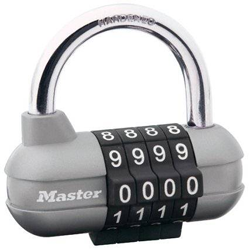
\includegraphics[scale=.5]{template/CombinacionDeLaCerradura/images/cerradura.png}
\end{figure}

La combinación de la cerradura está representada por $n$ discos giratorios con dígitos del $0$ al $9$ escritos en ellos. Scrooge McDuck tiene que girar algunos discos para que la combinación de dígitos en los discos forme la combinación secreta. Entonces, en un solo movimiento, puede girar un disco un dígito hacia adelante o hacia atrás. En particular, en un movimiento puede pasar del dígito $0$ al dígito $9$ y viceversa. ¿Qué número mínimo de acciones necesita para eso?

\inputText

La primera línea contiene un único número entero $n$ $(1 \le n \le 1000)$, el número de discos en la combinación de la cerradura.

La segunda línea contiene una cadena de $n$ dígitos, el estado original de los discos.

La tercera línea contiene una cadena de $n$ dígitos, la combinación de Scrooge McDuck que abre la cerradura.

\outputText

Imprime un único número entero, el número mínimo de movimientos que Scrooge McDuck necesita para abrir la cerradura.

\exampleCases

\begin{example}
    \exmp{%%INPUT
        \caseFile{template/CombinacionDeLaCerradura/in/1.in}
    }{%%OUTPUT
        \caseFile{template/CombinacionDeLaCerradura/out/1.out}
    }%%END-OUTPUT
        \exmp{%%INPUT
        \caseFile{template/CombinacionDeLaCerradura/in/2.in}
    }{%%OUTPUT
        \caseFile{template/CombinacionDeLaCerradura/out/2.out}
    }%%END-OUTPUT
\end{example}

\explanationText

En el primer ejemplo se necesita 13 movimientos:
\begin{itemize}
    \item 1 disco: $8 \longrightarrow 7 \longrightarrow 6$
    \item 2 disco: $2 \longrightarrow 3 \longrightarrow 4$
    \item 3 disco: $1 \longrightarrow 0 \longrightarrow 9 \longrightarrow 8 \longrightarrow 7$
    \item 4 disco: $9 \longrightarrow 0 \longrightarrow 1 \longrightarrow 2$
    \item 5 disco: $5 \longrightarrow 4 \longrightarrow 3$
\end{itemize}
